\documentclass[a4paper,12pt]{article}

\makeatletter
\providecommand\IfPDFManagementActiveF[2]{#2}
\makeatother

\usepackage{caption}
\captionsetup{font=footnotesize}
\usepackage[left=2.54cm, right=2.54cm, top=2.54cm, bottom=2.54cm]{geometry}
\usepackage[utf8]{inputenc} % para escribir full spanish
\usepackage{graphicx} % Required for inserting images
\usepackage{amsfonts}
\usepackage{lipsum}
\usepackage{minted}
\usepackage{csquotes}
\usepackage{makecell}
\usepackage{courier} 
\usepackage[usenames]{color} % todo esto es para los textos y las cosas de colores
\usepackage{tcolorbox}
\usepackage{color}
\usepackage{indentfirst}
\usepackage{xcolor}
\usepackage{svg} % para las imagenes vectorizadas
\definecolor{azul}{rgb}{0.17, 0.40, 0.71} % no me quiero aprender los numeritos 
\usepackage{listings}
\usepackage{amssymb} % para escribir cosas matemáticas 
\usepackage{amsmath} % para escribir más cosas matemáticas
\usepackage[english]{babel} % un rollo de traducciones de comandos al spanish
\renewcommand{\thesection}{\arabic{section}}
\usepackage{fancyhdr}
\usepackage{subfiles}
\usepackage{csquotes}
\usepackage{adjustbox}
\usepackage[hidelinks]{hyperref}
\usepackage{enumitem}
% \usepackage[backend=biber, style=verbose-trad2]{biblatex} % O el estilo que necesites (ej. 'authoryear-comp')
% \addbibresource{bibliografia.bib} % Sustituye por el nombre de tu archivo .bib

% Configuración de hyperref
\hypersetup{
    colorlinks=true,       % Activa el coloreado de los enlaces (quita los recuadros)
    urlcolor=blue,         % Color para URLs externas (\href)
    linkcolor=blue,        % Color para enlaces internos (como índices y referencias)
    citecolor=blue         % Color para citas bibliográficas
}
\lstdefinestyle{Python}{
  language=Python,
  basicstyle=\ttfamily\footnotesize, % letra más pequeña
  keywordstyle=\color{blue},
  commentstyle=\color{gray},
  stringstyle=\color{red},
  backgroundcolor=\color{gray!10}, % fondo gris claro
  showstringspaces=false,
  breaklines=true,
  frame=none, % sin marco
  captionpos=b
}
\lstset{style=Python}

% Pie de página
\pagestyle{fancy}
\fancyhf{}
\fancyfoot[C]{\thepage}

% Encabezado
\renewcommand{\headrulewidth}{0pt} % Definir el grosor de la línea a cero

% Para que no haya palabras entre márgenes
\hyphenpenalty=10000
\exhyphenpenalty=10000

\usepackage{csquotes}
\usepackage{adjustbox}
\usepackage[hidelinks]{hyperref}
\setlength{\parindent}{0cm}
\usepackage{graphicx}
\usepackage{subfigure}
% \usepackage{subcaption}
\renewenvironment{quote}
  {\vspace{-\topsep}\list{}{\rightmargin=0cm \leftmargin=1cm}%
   \item\relax}
  {\endlist\vspace{-\topsep}}

\setlength{\parindent}{20pt}

\begin{document}
\sloppy
\begin{titlepage}
    \vspace{40cm}

    \begin{center}
        \Huge \textsc{\textbf{Análisis deportivo mediante visión artificial aplicada al tenis}} \\
        \vspace{15mm}
        \Huge \textsc{Visión Artificial} \\
        \vspace{10mm}
        \textcolor{azul}{\rule{\linewidth}{0.55mm}}
        \vspace{3mm}
        \Large{
        \\
        \textbf{Ginés Carrillo Ibáñez}\\
          \vspace{3mm}
        \textbf{Yago Ibarrola Lapeña}\\
          \vspace{3mm}
        \textbf{Aarón Palomar Peña}\\
          \vspace{3mm}
        }
%\begin{center}
%    \includegraphics[width=0.5\textwidth]{}
%\end{center}

\begin{figure}[H]
    \centering
    \begin{minipage}[b]{0.4\textwidth}
        \centering
        
\includegraphics[width=0.8\textwidth]{portada/Escudo-UM-2023-sello (1).jpg}
    \end{minipage}
    \hfill
    \begin{minipage}[b]{0.4\textwidth}
        \centering
        
\includegraphics[width=0.8\textwidth]{portada/escudoFIUM.png}
    \end{minipage}
\end{figure}
    \vspace{3mm}
    Técnicas utilizadas: \\
    \vspace{3mm}
    \small{
    BT5a(5\%), BT5b(5\%), BT5c(5\%), BT5d(5\%), BT5e(5\%), BT5f(5\%), BT5g(5\%) \\
    }
    \vspace{30mm}
    {\large {Universidad de Murcia} \\}
        {\large {Facultad de Informática} \\}
            \vspace{5mm}
         {\large Curso 2025/2026}
          \vspace{10mm} \\
    \end{center}
\end{titlepage}
\renewcommand*\contentsname{Contenidos}
\addtocontents{toc}{\protect\setcounter{tocdepth}{-1}}
\tableofcontents
\thispagestyle{empty}
\addtocontents{toc}{\protect\setcounter{tocdepth}{2}}

\chapter{Sesión 1}
Para esta sesión, junto con la instalación de Nebula, se han realizado los 
siguientes experimentos con el entrenamiento de una CNN en el dataset CIFAR-10 
de clasificación de imágenes:
\begin{itemize}
    \item Entrenamiento usando FL centralizado con 
    \item Entrenamiento usando FL descentralizado
\end{itemize}
En los cuatro experimentos, se han realizado 10 rondas de entrenamiento en una única época. Se han desplegado 4 nodos y las actualizaciones se han calculado con FedAvg.


\section{FL centralizado}
Comparamos 
\section{Sesión 2}
% SESSION II: FL ATTACKS
Para esta sesión, se ha utilizado de nuevo la configuracion de entrenamiento de DFL non-IID de la sesión anterior. Se han realizado con ella los siguientes experimentos:
\begin{itemize}
    \item Ataque de \textit{model poisoning} con 10\% de ruido gaussiano.
    \item Ataque de \textit{label flipping} con 80\% de muestras envenenadas.
\end{itemize}
Para cada uno de los ataques, compararemos con un 20\% y un 50\% de clientes maliciosos. 


\subsection{Model poisoning}

En este ataque, los clientes maliciosos añaden ruido gaussiano a sus modelos locales antes de enviarlos para la agregación. Este ruido degrada la calidad de las actualizaciones, afectando al proceso de convergencia.
\vspace{1mm}

Los resultados obtenidos se muestran en la Figura \ref{fig:model_poisoning}:

\vspace{1mm}
\noindent
\begin{minipage}{\textwidth}
    \centering
    \begin{tabular}{cc}
        \textbf{20\% nodos maliciosos} & \textbf{50\% nodos maliciosos} \\
        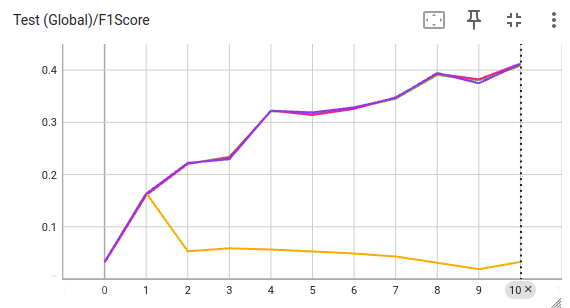
\includegraphics[width=0.4\textwidth]{images/model_poisoning_20.png} &
        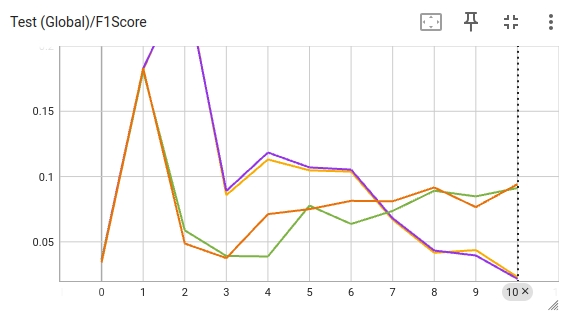
\includegraphics[width=0.4\textwidth]{images/model_poisoning_50.png} \\
    \end{tabular}
    \captionof{figure}{Impacto del ataque de \textit{model poisoning} con diferentes porcentajes de nodos maliciosos.}
    \label{fig:model_poisoning}
\end{minipage}
\vspace{1mm}

Se observa que el impacto del ataque aumenta significativamente con el número de nodos maliciosos, provocando una notable inestabilidad:

\begin{itemize}
    \item Con un 20\% de nodos maliciosos, la mayoría de los participantes logra converger hacia un F1-score aproximado de 0.41. Sin embargo, el nodo atacante queda rezagado con un valor de apenas 0.03 porque realiza el test después de introducir el ruido al modelo recibido por el agregador.
    \item Con un 50\% de nodos maliciosos, la convergencia se ve gravemente afectada. La gráfica muestra fuertes oscilaciones y una degradación final, desplomando el F1-score a valores casi nulos de entre 0.02 y 0.09 en el último paso.
\end{itemize}

%Las matrices de confusión reflejan un aumento en los errores de clasificación generalizados, sin afectar a clases específicas de forma predominante, lo cual es consistente con la naturaleza no dirigida del ruido gaussiano.

\subsection{Label flipping}

En este caso, los nodos maliciosos alteran las etiquetas de un 80\% de sus muestras de entrenamiento de manera aleatoria. Este ataque introduce información incorrecta directamente en el proceso de aprendizaje.
\vspace{1mm}

Los resultados se muestran en la Figura \ref{fig:label_flipping}:

\vspace{1mm}
\noindent
\begin{minipage}{\textwidth}
    \centering
    \begin{tabular}{cc}
        \textbf{20\% nodos maliciosos} & \textbf{50\% nodos maliciosos} \\
        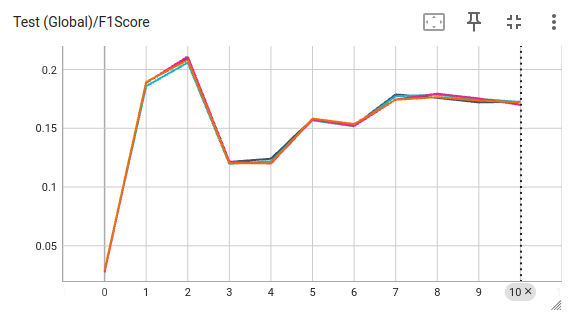
\includegraphics[width=0.4\textwidth]{images/label_flipping_20.png} &
        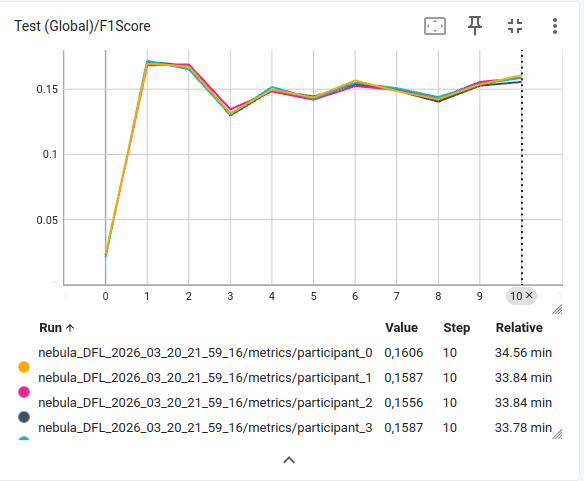
\includegraphics[width=0.4\textwidth]{images/label_flipping_50.png} \\
    \end{tabular}
    \captionof{figure}{Impacto del ataque de \textit{label flipping} con diferentes porcentajes de nodos maliciosos.}
    \label{fig:label_flipping}
\end{minipage}
\vspace{1mm}

En este escenario, el impacto reduce el rendimiento pero mantiene un entrenamiento más estable:

\begin{itemize}
    \item Con un 20\% de nodos maliciosos, el modelo presenta una convergencia estable agrupada para todos los clientes, alcanzando un F1-score final en torno a 0.48.
    \item Con un 50\% de nodos maliciosos, el modelo logra converger pero el rendimiento se desploma, estancándose de manera uniforme en un F1-score de 0.15.
\end{itemize}

%Las matrices de confusión muestran patrones de error más estructurados, con confusión sistemática entre clases, lo que indica que el modelo aprende relaciones incorrectas debido a las etiquetas alteradas.

\subsection{Comparación y análisis}

Comparando ambos ataques y configuraciones con los datos obtenidos, se extraen las siguientes conclusiones:

\begin{itemize}
    \item Contrario a lo que se podría intuir en un inicio, el ataque de \textit{model poisoning} genera un escenario más desestabilizador y destructivo en altas proporciones (50\%) que el de \textit{label flipping}. Mientras el primero destruye la convergencia (F1-score $\leq 0,09$), el segundo logra engañar al modelo llevándolo a una convergencia falsa pero ligeramente superior (F1-score $\sim 0,16$).
    \item A medida que aumenta el porcentaje de clientes maliciosos (20\% $\rightarrow$ 50\%), la métrica final cae drásticamente en ambos ataques: de $\sim$0,41 a $\leq$0,09 en \textit{model poisoning}, y de $\sim$0,48 a $\sim$0,16 en \textit{label flipping}.
    %\item En comparación con los resultados de la sesión 1, donde el caso non-IID ya presentaba dificultades de convergencia, los ataques agravan aún más este problema y resaltan la fragilidad de estas redes frente a actores bizantinos.
    \item En la sesión anterior, el entorno DFL ideal (IID) alcanzaba un F1-score de $\sim$0,67, mientras que la simple introducción de heterogeneidad en los datos (DFL non-IID base) lo reducía a $\sim$0,50. Al introducir condiciones de ataque sobre este último escenario, la degradación se amplifica: en la condición de ataque más leve (20\% \textit{label flipping}), el F1-score ya cae por debajo del caso base a $\sim$0,48. En las condiciones de ataque más severas (50\% \textit{model poisoning}), el modelo se desploma hasta un 0,02. Esto evidencia que los entornos non-IID son frágiles ante actualizaciones maliciosas, ya que a la agregación le resulta mucho más difícil distinguir entre una variación legítima (datos sesgados) y un ataque intencionado.

\end{itemize}

% En cuanto a la evolución temporal:

% \begin{itemize}
%     \item En escenarios de \textit{model poisoning} se evidencia un claro comportamiento errático (oscilaciones abruptas en el caso del 50\%) y particiones en el aprendizaje global (como el nodo rezagado en el caso del 20\%).
%     \item El \textit{label flipping}, por el contrario, fomenta una ilusión de estabilidad, ya que todos los participantes convergen de manera solidaria pero hacia un modelo que ha interiorizado lógicas de clasificación erróneas.
% \end{itemize}

% En resumen, los ataques afectan tanto a la calidad final del modelo como a la dinámica de entrenamiento, siendo el entorno non-IID especialmente vulnerable debido a la ya existente heterogeneidad de los datos.

Matriz de atacante
\section{Sesión 3}
% SESSION III: DEFENSE AGAINST ADVERSARIAL ATTACKS IN FL

Para esta sesión, se ha utilizado de nuevo la configuración de entrenamiento DFL non-IID con la presencia de un nodo malicioso realizando \textit{model poisoning}, tal y como se definió en la sesión anterior. Sobre este escenario, se han evaluado dos mecanismos de agregación robusta con el objetivo de mitigar el impacto de actualizaciones adversarias:

\begin{itemize}
    \item Agregación mediante \textit{Trimmed Mean}.
    \item Agregación mediante \textit{Krum}.
\end{itemize}

\subsection{Trimmed Mean}

El algoritmo \textit{Trimmed Mean} consiste en eliminar un porcentaje de los valores más extremos (potencialmente maliciosos) antes de realizar la agregación de los modelos, reduciendo así la influencia de outliers.

\vspace{1mm}

Los resultados se muestran en la Figura \ref{fig:trimmed_mean}:

\vspace{1mm}
\noindent
\begin{minipage}{\textwidth}
    \centering
    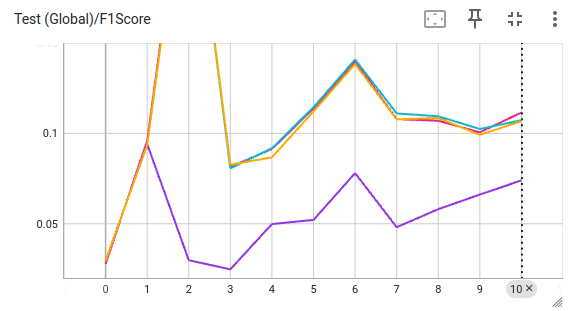
\includegraphics[width=0.5\textwidth]{images/trimmed_mean.png}
    \captionof{figure}{Resultados del entrenamiento con agregación \textit{Trimmed Mean}.}
    \label{fig:trimmed_mean}
\end{minipage}
\vspace{1mm}

Se observa que este método consigue mitigar parcialmente el efecto del nodo malicioso:

\begin{itemize}
    \item El modelo converge de manera relativamente estable, evitando las oscilaciones bruscas observadas en \textit{model poisoning} sin defensa.
    \item El F1-score final se sitúa en torno a 0.11--0.12, lo que supone una mejora significativa frente al caso atacado sin mecanismos de defensa.
    \item Sin embargo, el rendimiento sigue siendo inferior al escenario sin ataques, indicando que el filtrado de valores extremos no elimina completamente el impacto adversario.
\end{itemize}

% Las matrices de confusión muestran una mejora global en la clasificación respecto al escenario atacado, aunque persisten errores distribuidos entre varias clases.

Punto clave: TrimmedMean usa beta=0 por defecto en trimmedmean.py:15, y no vi que backend lo configure. Con beta=0, no recorta extremos y termina en media simple por componente en trimmedmean.py:37.
Además, ese TrimmedMean no pondera por tamaño de dataset (solo promedia tensores), mientras FedAvg sí pondera por muestras en fedavg.py:23 y fedavg.py:33.
Krum aquí selecciona un único modelo (el de menor suma de distancias) en krum.py:44 y krum.py:49; no pondera por muestras y puede tirar mucha información útil en non-IID.


\subsection{Krum}

El algoritmo \textit{Krum} selecciona la actualización más representativa entre los nodos, basándose en la distancia entre modelos, con el objetivo de descartar aquellos que se alejan significativamente (potencialmente maliciosos).

\vspace{1mm}

Los resultados se presentan en la Figura \ref{fig:krum}:

\vspace{1mm}
\noindent
\begin{minipage}{\textwidth}
    \centering
    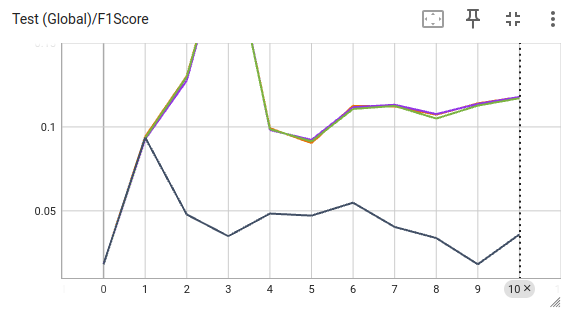
\includegraphics[width=0.5\textwidth]{images/krum.png}
    \captionof{figure}{Resultados del entrenamiento con agregación \textit{Krum}.}
    \label{fig:krum}
\end{minipage}
\vspace{1mm}

En este caso, el comportamiento es diferente:

\begin{itemize}
    \item El entrenamiento es más estable que en el caso sin defensa, pero presenta mayor variabilidad que \textit{Trimmed Mean}.
    \item El F1-score final se sitúa aproximadamente entre 0.07 y 0.11 dependiendo del nodo, mostrando un rendimiento ligeramente inferior en promedio.
    \item Esto sugiere que, aunque Krum es capaz de descartar actualizaciones maliciosas, puede verse afectado por la heterogeneidad non-IID, seleccionando modelos que no representan adecuadamente la distribución global.
\end{itemize}

% Las matrices de confusión reflejan una mayor dispersión en los errores, indicando que el modelo puede estar sesgado hacia ciertas clases dependiendo del nodo seleccionado en cada ronda.

\subsection{Comparación y análisis}

A partir de los resultados obtenidos, se pueden extraer las siguientes conclusiones:

\begin{itemize}
    \item \textit{Trimmed Mean} demuestra una mayor robustez frente a ataques de \textit{model poisoning}, ya que consigue estabilizar la convergencia y alcanzar un F1-score superior en promedio.
    % \textbf{Mayor resiliencia:} 
    \item En escenarios con datos heterogéneos, \textit{Krum} puede verse penalizado, ya que la variabilidad entre nodos puede confundirse con comportamiento malicioso, afectando negativamente a la selección de modelos.
    % \textbf{Impacto de non-IID:} 
    %\item Ninguno de los métodos elimina completamente el efecto del atacante. En \textit{Krum}, se observa un mayor sesgo hacia ciertas clases, lo que sugiere un posible sobreajuste local dependiendo del nodo seleccionado. En \textit{Trimmed Mean}, los errores son más uniformes, indicando un comportamiento más equilibrado.
    % \textbf{Rendimiento por clases:} 
    \item  Ambos métodos mejoran claramente el rendimiento respecto al escenario atacado sin defensa (F1-score $\leq 0.09$), pero no alcanzan los niveles del escenario sin ataques. Esto confirma que, aunque las técnicas robustas ayudan, no eliminan completamente el efecto adversarial.
    % \textbf{Comparación global:}
\end{itemize}

%En conjunto, \textit{Trimmed Mean} resulta más adecuado en este escenario concreto, al ofrecer un mejor equilibrio entre robustez y estabilidad en presencia de nodos maliciosos y datos non-IID.
\section{Sesión 4}

% En esta sesión estamos interesados en la evaluación de distintos mecanismos de reputación. Con este propósito,
% se ha utilizado una la configuración de entrenamiento DFL non-IID con la presencia de un nodo malicioso 
% realizando un \textit{flooding attack}. Sobre este escenario, se han usado dos configuraciones de reputación diferentes:

% \begin{itemize}
%     \item Reputación mediante \textit{pesos estáticos}.
%     \item Reputación mediante \textit{pesos dinámicos}.
% \end{itemize}

% En ambos casos, la reputación inicial de cada nodo se ha establecido en 0.5. Los pesos hacen referencia a la importancia
% relativa de cada métrica usada. En nuestro caso, usaremos siempre las 4 métricas disponibles, que se dividen en dos categorías:
% \textbf{métricas basadas en el modelo}, que incluyen \textit{Similitud del modelo} y \textit{Fracción de parámetros cambiados}, y
% \textbf{métricas basadas en la comunicación}, que incluyen \textit{Número de mensajes} y \textit{Latencia de llegada del modelo}.
% \vspace{1mm}

% En el caso del ataque de \textit{flooding}, el nodo malicioso trata de saturar la red. El sistema de reputación
% debe ser capaz de identificar este comportamiento anómalo y reducir la influencia del nodo atacante en el proceso
% de aprendizaje.

\subsection{Pesos estáticos}

% En esta configuración, se asignan pesos fijos a cada métrica para calcular la reputación de los nodos. Este método
% es muy sencillo pero poco flexible. Los pesos asignados son 0.30 / 0.15 / 0.30 / 0.25.

% \vspace{1mm}

Las reputaciones calculadas por cada nodo se muestran en la Figura \ref{fig:reputation_static}:

\vspace{1mm}
\noindent
\begin{minipage}{\textwidth}
    \centering
    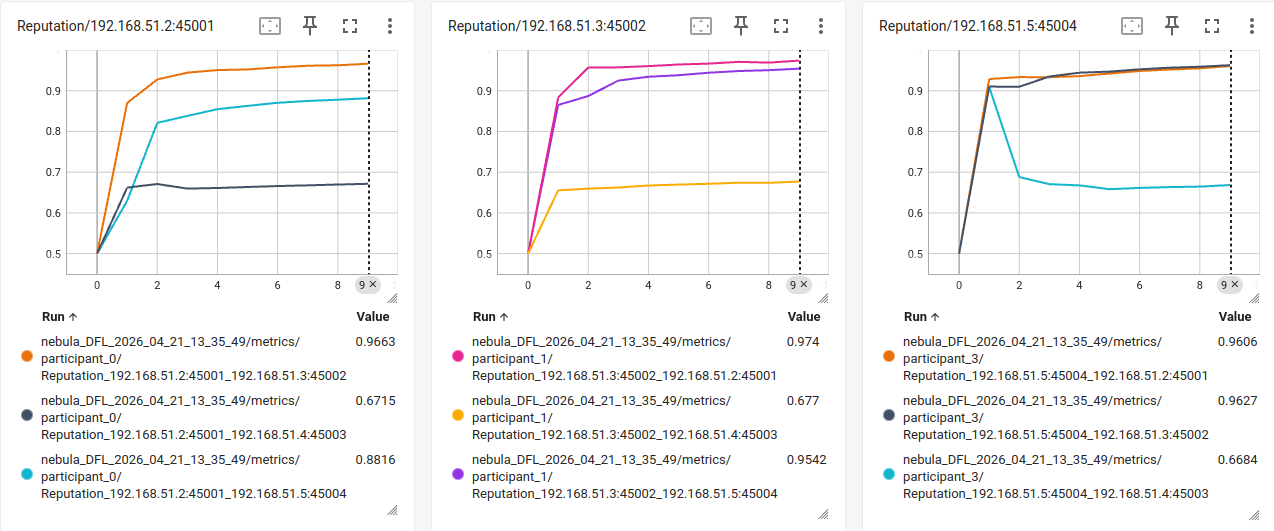
\includegraphics[width=0.9\textwidth]{images/reputation_static_rep.png}
    \captionof{figure}{Reputación con pesos estáticos a lo largo del entrenamiento.}
    \label{fig:reputation_static}
\end{minipage}
\vspace{1mm}

Vemos que los tres nodos honestos otorgan una reputación inferior al nodo malicioso.
Desde el punto de vista de cada nodo honesto, los demás nodos honestos tienen una
reputación muy cercana a 1, mientras que la reputación del nodo malicioso es algo
inferior a 0.7. Esta diferencia coincide con la poderación de la métrica de número
de mensajes (0.3), en la que el nodo malicioso obtiene una puntuación terrible (envía
alrededor de 15 mensajes por ronda). Dado que el nodo malicioso obtiene una buena puntuación
en las otras métricas, su reputación total se mantiene por encima de 0.5 y el nodo malicioso
se sigue considerando como honesto.

En cuanto a los resultados del entrenamiento con esta configuración, se muestran en la Figura \ref{fig:reputation_static_results}:
\vspace{1mm}

\begin{figure}[htbp]
    \centering
    % Primera imagen: f1
    \begin{minipage}{0.3\textwidth}
        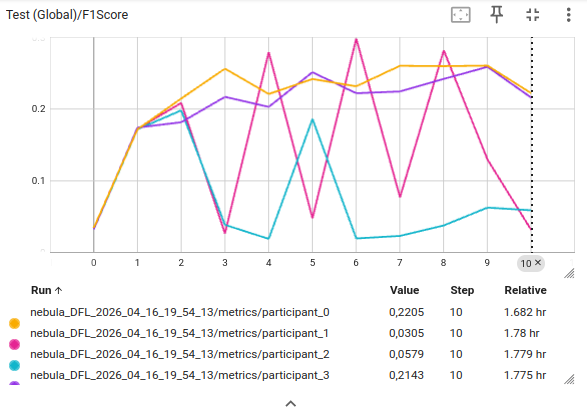
\includegraphics[width=\textwidth]{images/reputation_static_f1.png}
    \end{minipage}
    \hfill
    % Segunda imagen: cm
    \begin{minipage}{0.25\textwidth}
        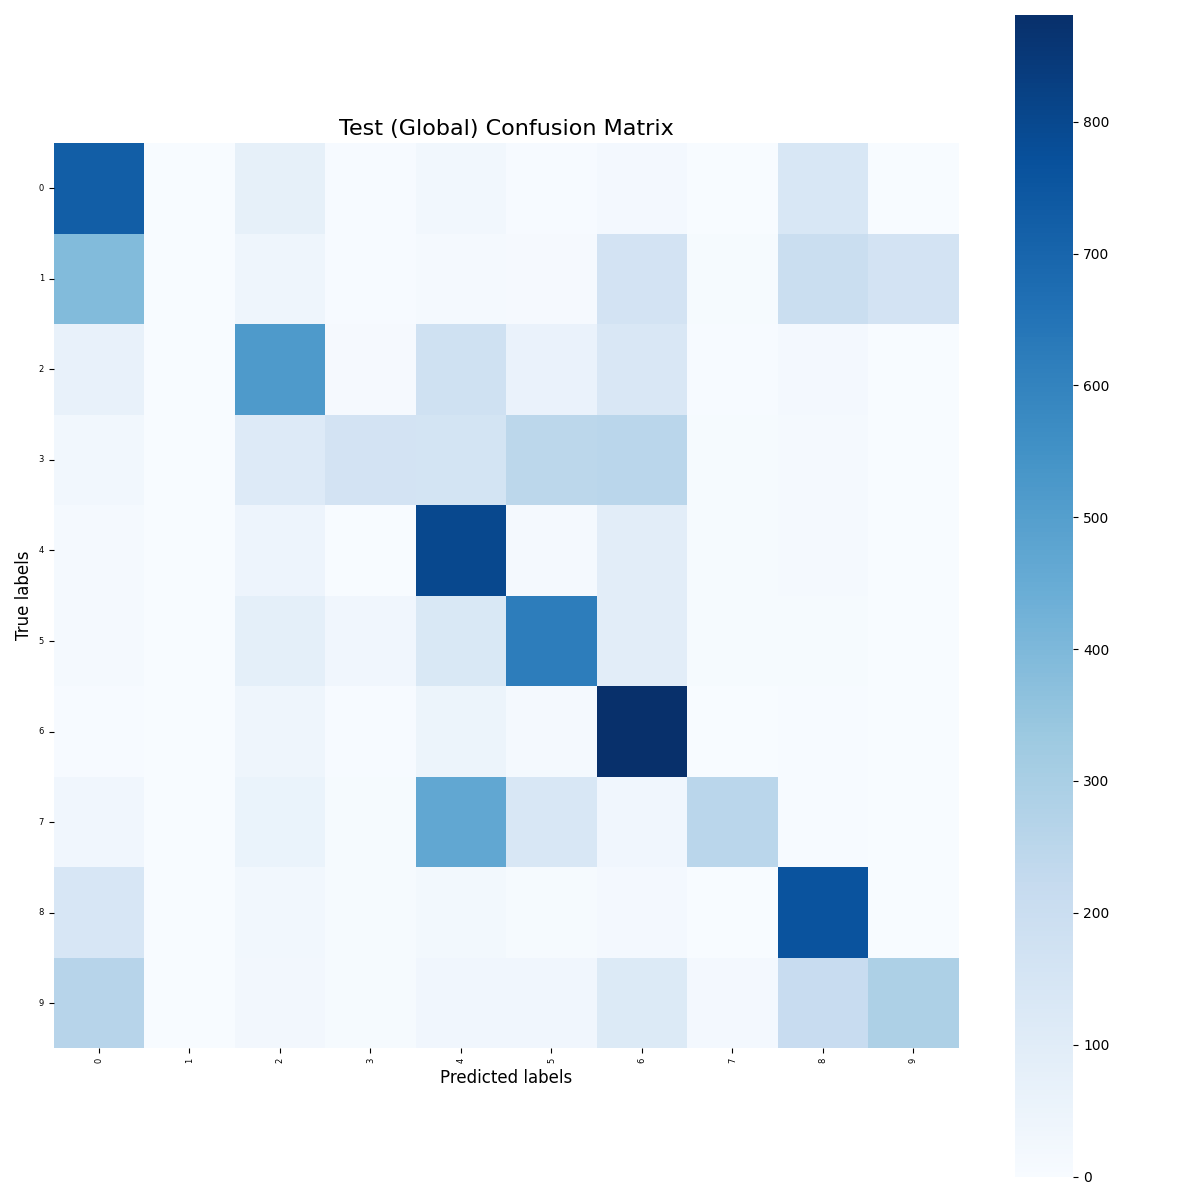
\includegraphics[width=\textwidth]{images/reputation_static_cm_honest.png}
    \end{minipage}
    \hfill
    % Tercera imagen: cm2
    \begin{minipage}{0.25\textwidth}
        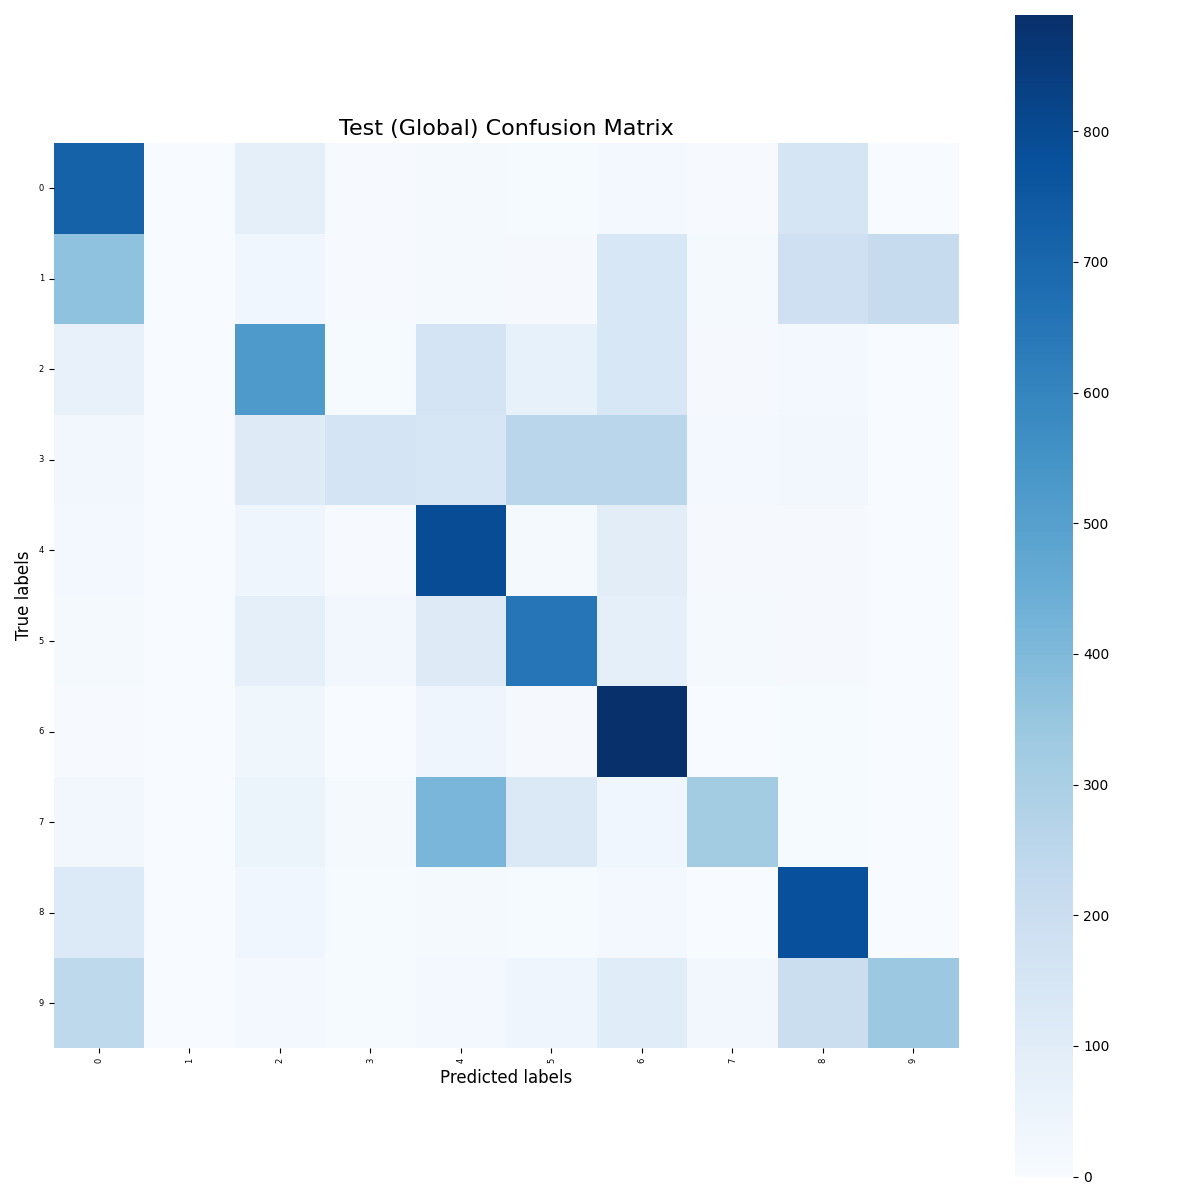
\includegraphics[width=\textwidth]{images/reputation_static_cm_malicious.png}
    \end{minipage}
    
    \caption{Resultados del entrenamiento con pesos estáticos: F1-score y matrices de confusión. Matriz de confusión del nodo malicioso a la derecha.}
    \label{fig:reputation_static_results}
\end{figure}

%REVISAR LA PRIMERA PARTE DE ESTE PÁRRAFO
La gráfica del F1-score apenas muestra señales del ataque. Los modelos alcanzan un F1-score cercano a 0.46,
mientras que el baseline (sin ataque) alcanza alrededor de 0.49. Esto es debido a que, a pesar del ataque 
de flooding, el contenido de los mensajes del nodo malicioso es correcto. El ataque resulta en un aumento del tráfico,
lo que si hace que el tiempo de entrenamiento esté cerca de duplicarse (4 minutos baseline vs 8 minutos con flooding y pesos estáticos).
Parte de este overhead puede ser debido también a la gestión de la reputación.
En cuanto a las matrices de confusión, las cuatro resultantes son prácticamente idénticas, lo que indica que los modelos han convergido.
A la izquierda se muestra la matriz de confusión de un nodo honesto y a la derecha la del nodo malicioso.

\subsection{Pesos dinámicos}

% En esta configuración, los pesos se ajustan dinámicamente para cada métrica en
% función de las condiciones del entorno.

% \vspace{1mm}

Los resultados se presentan en la Figura \ref{fig:reputation_dynamic}:

\vspace{1mm}
\noindent
\begin{minipage}{\textwidth}
    \centering
    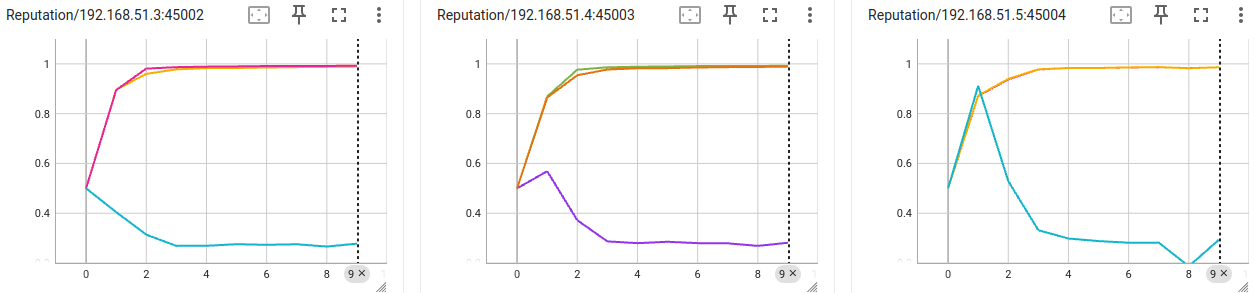
\includegraphics[width=0.9\textwidth]{images/reputation_dynamic_rep.png}
    \captionof{figure}{Reputación con pesos dinámicos a lo largo del entrenamiento.}
    \label{fig:reputation_dynamic}
\end{minipage}
\vspace{1mm}

En este caso, se observa que los nodos honestos asignan una reputación mucho más baja al nodo malicioso.
Esta vez la reputación del nodo malicioso cae hasta aproximadamente 0.3. Este valor, al quedar por debajo de 0.5, causa
la exclusión de las actualizaciones del nodo malicioso en el proceso de agregación. Sin embargo, parece que sí se le
siguen enviando las actualizaciones del modelo global, lo que permite que el nodo malicioso siga aprendiendo y mejorando
su rendimiento.
Los resultados del entrenamiento con esta configuración se muestran en la Figura \ref{fig:reputation_dynamic_results}:

\vspace{1mm}
\begin{figure}[htbp]
    \centering
    % Primera imagen: f1
    \begin{minipage}{0.3\textwidth}
        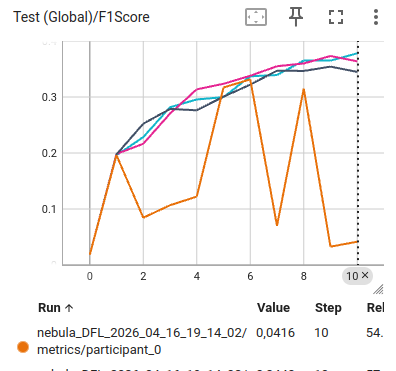
\includegraphics[width=\textwidth]{images/reputation_dynamic_f1.png}
    \end{minipage}
    \hfill
    % Segunda imagen: cm
    \begin{minipage}{0.25\textwidth}
        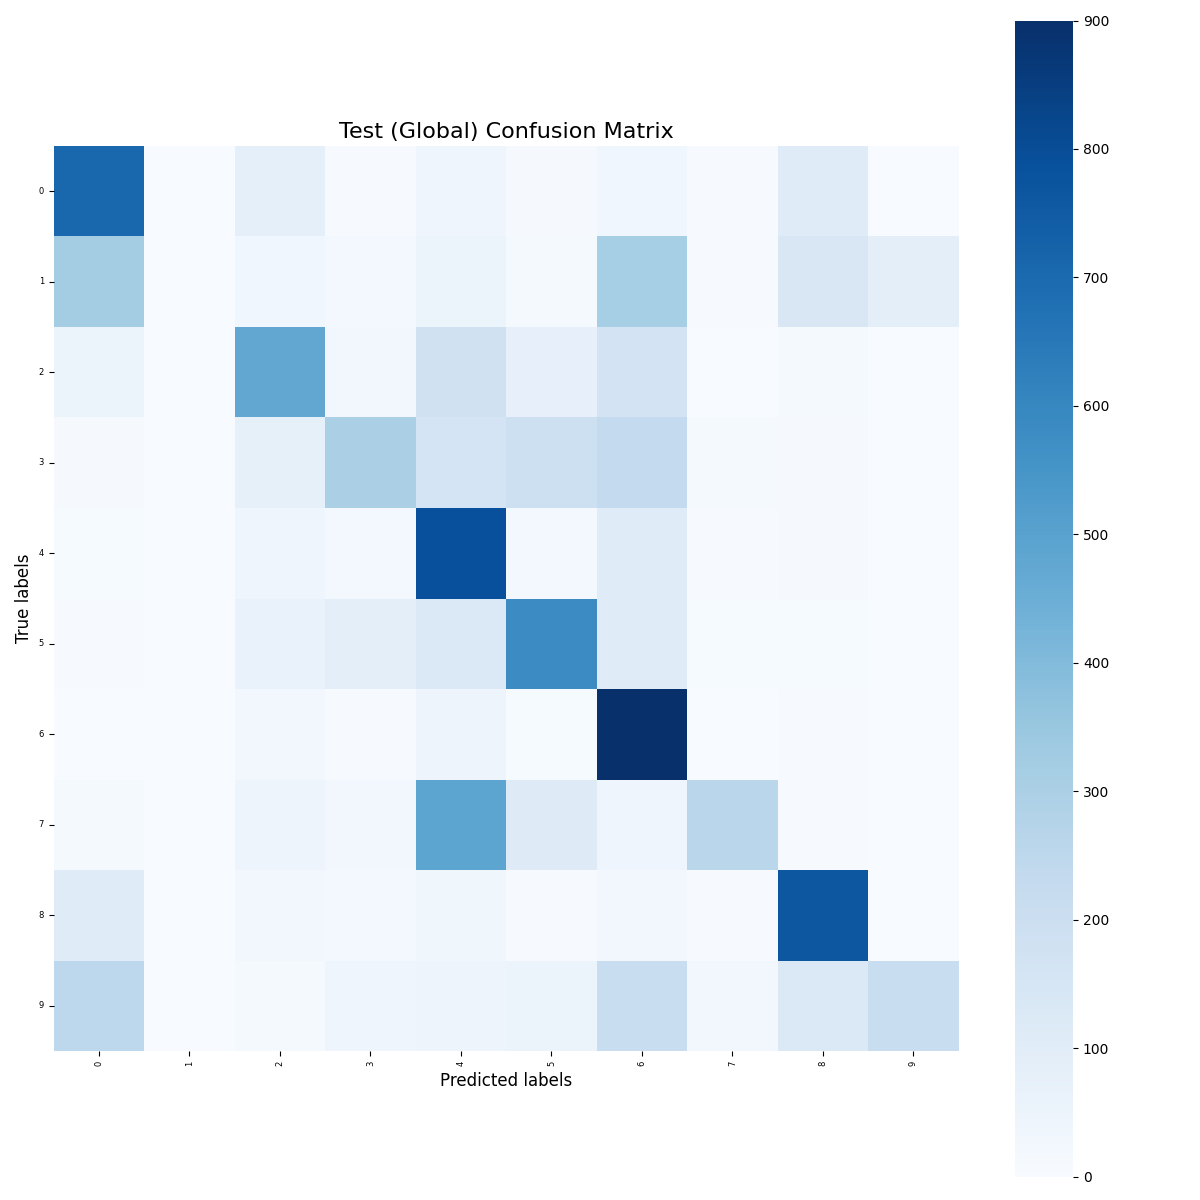
\includegraphics[width=\textwidth]{images/reputation_dynamic_honest_cm.png}
    \end{minipage}
    \hfill
    % Tercera imagen: cm2
    \begin{minipage}{0.25\textwidth}
        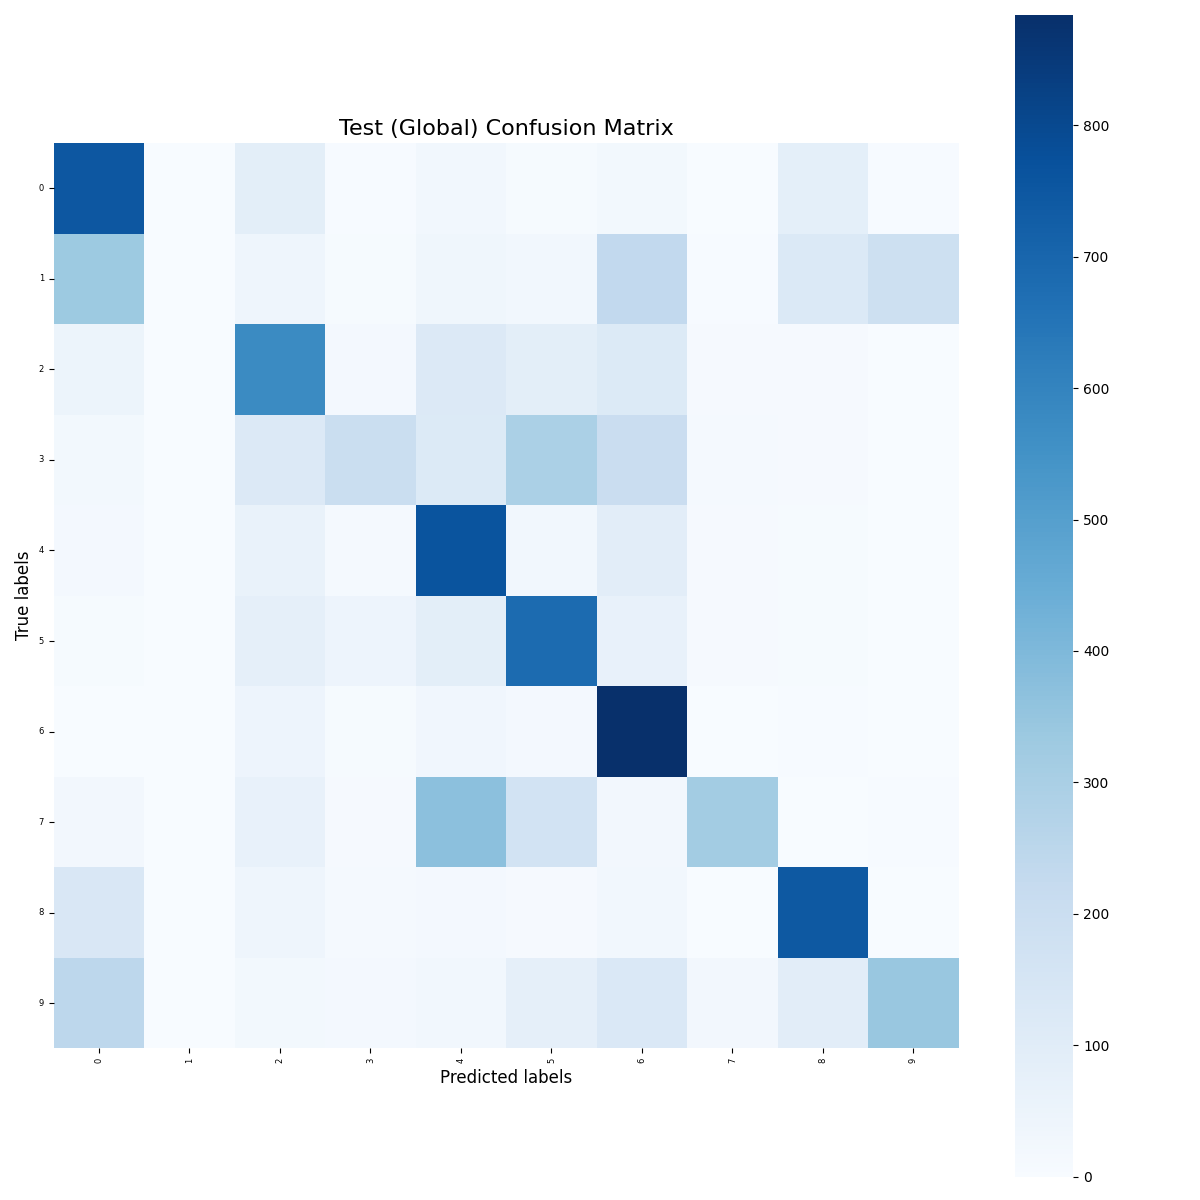
\includegraphics[width=\textwidth]{images/reputation_dynamic_malicious_cm.png}
    \end{minipage}
    
    \caption{Resultados del entrenamiento con pesos dinámicos: F1-score y matrices de confusión. Matriz de confusión del nodo malicioso a la derecha.}
    \label{fig:reputation_dynamic_results}
\end{figure}

La gráfica de F1-score es también similar a la anterior. Resulta curioso que el nodo malicioso obtenga un rendimiento
incluso mejor que el resto, lo que se debe a que es el único que sigue utilizando sus datos para entrenar (al tener
baja reputación, los otros nodos descartan sus actualizaciones). Esto, irónicamente, aporta cierta ventaja al nodo malicioso. El tiempo de
entrenamiento es muy similar al de la configuración de pesos estáticos. Esto puede ser debido a que el nodo malicioso
sigue enviando y recibiendo mensajes, aunque estos sean ignorados posteriormente.
En cuanto a las matrices de confusión, la de la izquierda es de un nodo honesto, mientras que la de la derecha corresponde
al nodo malicioso. De nuevo, los modelos convergen y las cuatro matrices de confusión son prácticamente idénticas.

\subsection{Comparación y análisis}

A partir de los resultados obtenidos, se pueden extraer las siguientes conclusiones:

\begin{itemize}
    \item La reputación con \textit{pesos dinámicos} demuestra una mayor capacidad de detección de ataques de \textit{flooding}, y cabe esperar que también sea superior a \textit{pesos estáticos} frente a otros tipos de ataques.
    \item Solo en el escenario con pesos dinámicos, el nodo malicioso es detectado y excluido completamente. Esta exclusión ocurre ya en la segunda ronda.
    \item La reacción de la federación ante el ataque es completamente ineficaz, incluso al detectarlo completamente. De hecho, la detección y exclusión de este causan que el modelo del
    atacante obtenga mejores resultados que los demás, cosa que no ocurriría si el ataque no fuera detectado.
\end{itemize}

%En conjunto, \textit{Trimmed Mean} resulta más adecuado en este escenario concreto, al ofrecer un mejor equilibrio entre robustez y estabilidad en presencia de nodos maliciosos y datos non-IID.

% ◼  Which configuration (static or dynamic) offered the best balance between robustness and 
% learning accuracy? 
% ◼  Did the reputation system detect and isolate malicious nodes early during training or from a 
% specific round?

% \newpage
% \bibliographystyle{plainurl}
% \bibliography{bibliografia}
\end{document}